\documentclass{article}
\usepackage{CS4F_Colors}
\usepackage{csff}

% xelatex und biber
% Defintion für das Datum hier eingeben
\def \dokumentdatum {Februar 2024}


\graphicspath{ {../../Figures/}}

\title{Energieeffizienz\\im digitalen Alltag und beim Coding\\[2mm]Wissenschaftlicher Hintergrund} 
\author{Julia Padberg und Martin Becke}
\date{\dokumentdatum}

\begin{document}

\maketitle
\tableofcontents

\section{Einleitung}
Softwareentwicklung ist inzwischen ein zentraler Bestandteil des technologischen Fortschritts. Jedoch wird zunehmend erkannt, dass die digitale Technologien signifikant zu globalen Treibhausgasemissionen beitragen. Allein im Jahr 2020  wurden laut IEA\footnote{%
	               Internationale Energieagentur \href{https://www.iea.org/}{https://www.iea.org/}} 
330 Megatonnen CO$_2$-Äquivalente\cite{iea_digitalisation_tracking} durch Rechenzentren, Datenübertragungsnetzwerke und vernetzte Geräte emittiert. Vor diesem Hintergrund wird das ambitionierte Ziel verfolgt, diese Emissionen bis 2030 zu halbieren, um den Weg zur Netto-Null-Emission bis 2050 zu ebnen.

Diese Ausarbeitung zeigt eine Umsetzung aus den abstrakten Fakten zur CO$_2$-Emissionsreduktion\footnote{%
          Im folgenden sprechen wir von CO$_2$ auch, wenn es sich um andere Treibhausgase 
					oder  CO$_2$-Äquivalente handelt.}
von IT aus der Perspektive eines programmierenden Menschens auf. 
Diese Arbeit beleuchtet sowohl mögliche Maßnahmen im Alltag  und deren Auswirkungen auf die Emissionsreduktion als auch die Entwicklung von CO$_2$-effizienten Anwendungen in der Softwareentwicklung und deren Beitrag zur Emissionsminderung.

\section{Stand der Forschung zu CO$_2$-Emissionen}
 \subsection*{IEA}
  Laut der IEA wird der Klimawandel und seine Folgen ein unvermeidbares Thema für alle Disziplinen darstellen, einschließlich der Informatik. Die Studie \textit{Net Zero Roadmap} \cite{iea_net_zero2023} untersucht den aktuellen Stand der Netto-Null-Roadmap, wie sie von der IEA präsentiert wird. Insbesondere wird der Fokus auf saubere Energietechnologien gelegt, die die Aussichten für Emissionen durch politische Maßnahmen, expandierende Märkte und sinkende Kosten verändern. Trotz der aktuellen politischen Rahmenbedingungen wird erwartet, dass diese Technologien zu einer Verringerung der Emissionen um 7,5 Gigatonnen bis 2030 führen, basierend auf dem Basisszenario vor dem Pariser Abkommen von 2015.
	
Die voranschreitende Entwicklung sauberer Energietechnologien spielt eine entscheidende Rolle bei der Eindämmung von Treibhausgasemissionen. Politische Maßnahmen, expandierende Märkte und sinkende Kosten tragen dazu bei, dass Technologien wie Photovoltaik und Windkraft verstärkt genutzt werden. Im Szenario STEPS (Stated Policies Scenario) wird erwartet, dass der Ausbau von Photovoltaik und Windkraft um 5 Gigatonnen sowie die Integration von Elektrofahrzeugen für eine Reduktion von fast 1 Gigatonne verantwortlich sind.

Die Prognose einer Verringerung der Emissionen um 7,5 Gigatonnen bis 2030 im Vergleich zum Basisszenario vor dem Pariser Abkommen von 2015 ist von erheblicher Bedeutung. Dies verdeutlicht nicht nur den Fortschritt in der Umsetzung sauberer Energietechnologien, sondern auch die Wirksamkeit politischer Maßnahmen. Die Netto-Null-Roadmap bietet somit einen klaren Weg zur Erreichung der Emissionsziele.

Trotz der vielversprechenden Entwicklungen bleibt die prognostizierte Erwärmung von 2,4 Grad Celsius im Jahr 2100 besorgniserregend hoch. Dies verdeutlicht die Dringlichkeit weiterer Anstrengungen und innovativer Maßnahmen, um die Klimaerwärmung einzudämmen. Es ist jedoch zu betonen, dass die aktuelle Prognose um 1 Grad Celsius niedriger liegt als vor dem Pariser Abkommen von 2015, was auf die positiven Auswirkungen der implementierten Maßnahmen hinweist.
\newpage
\begin{figure}
		\includegraphics[width=1.00\textwidth]{../Figures/global-energy-sector-CO2-emissions-in-the-pre-paris-baseline-and-stated-policies-scenarios-2015-2030.png}
	\caption{Prognose der IEA (aus \cite{iea_net_zero2023PDF} S.25)
	\label{fig:global-energy-sector-CO2-emissions}}
\end{figure}
%
Die Abb.~\ref{fig:global-energy-sector-CO2-emissions} ~ illustriert die zukünftige Entwicklungen;  bis 2030 könnten, basierend auf dem Basisszenario des Pariser Abkommens von 2015 und unter der Annahme der Umsetzung politischer Maßnahmen, Emissionsverringerungen von etwa 7,5 Gigatonnen erreicht werden. Ein beachtlicher Teil dieser Reduktion, etwa fünf Gigatonnen, wird voraussichtlich durch den Ausbau von Photovoltaik und Windkraft erzielt. Zudem wird eine weitere Reduktion von einer Gigatonne durch den zunehmenden Einsatz von Elektrofahrzeugen erwartet.

Trotz dieser Fortschritte wird prognostiziert, dass, falls die derzeitigen Trends fortgesetzt werden, die globale Temperatur bis zum Jahr 2100 um 2,4 Grad Celsius ansteigen könnte. Diese Prognose, basierend auf Daten der Internationalen Energieagentur, ist zwar niedriger als die Interpolation von 2015, bleibt jedoch deutlich über dem gewünschten Ziel. 


 \subsection*{IPCC}
Das IPCC\footnote{%
         Intergovernmental Panel on Climate Change (Zwischenstaatlicher Ausschuss für Klimaänderungen)
				\href{https://www.ipcc.ch/}{https://www.ipcc.ch/}} 
wurde im Jahr 1988 von der Weltmeteorologieorganisation (WMO) der Vereinten Nationen (UN) und dem Umweltprogramm der Vereinten Nationen (UNEP) gegründet. Das IPCC hat die Aufgabe, wissenschaftliche Informationen über den Klimawandel zu bewerten und diese Bewertungen den politischen Entscheidungsträgern weltweit zur Verfügung zu stellen.
Eines der Hauptziele des IPCC ist die 
Bewertung des aktuellen wissenschaftlichen Wissens. Das IPCC sammelt und bewertet die neuesten wissenschaftlichen Erkenntnisse zum Klimawandel. Dies umfasst Informationen über den aktuellen Stand des Klimas, die Ursachen des Klimawandels, die Auswirkungen auf die Umwelt, die Gesellschaft und die Wirtschaft sowie mögliche Anpassungs- und Minderungsstrategien.



Die IEA fokussiert sich auf eine positivere Darstellung der Entwicklung, während das IPCC eine  dringlichere Sichtweise einnimmt, was die Notwendigkeit für sofortige Handlungen unterstreicht. Diese Diskrepanz in der Darstellung hebt die Komplexität und die Herausforderungen bei der Interpretation von Klimadaten hervor.
Des Weiteren zeigt eine Analyse des IPCC noch drastischere Szenarien. Die aktuellen Trends deuten darauf hin, dass selbst bei umfassenden Maßnahmen zur Emissionsreduktion eine Erwärmung von 1,5 bis 2 Grad unvermeidlich erscheint. Die Notwendigkeit, das Ziel von Net Zero – keine Emission von Treibhausgasen – zu erreichen, wird somit umso dringlicher.

\begin{figure}[h]
	\centering
		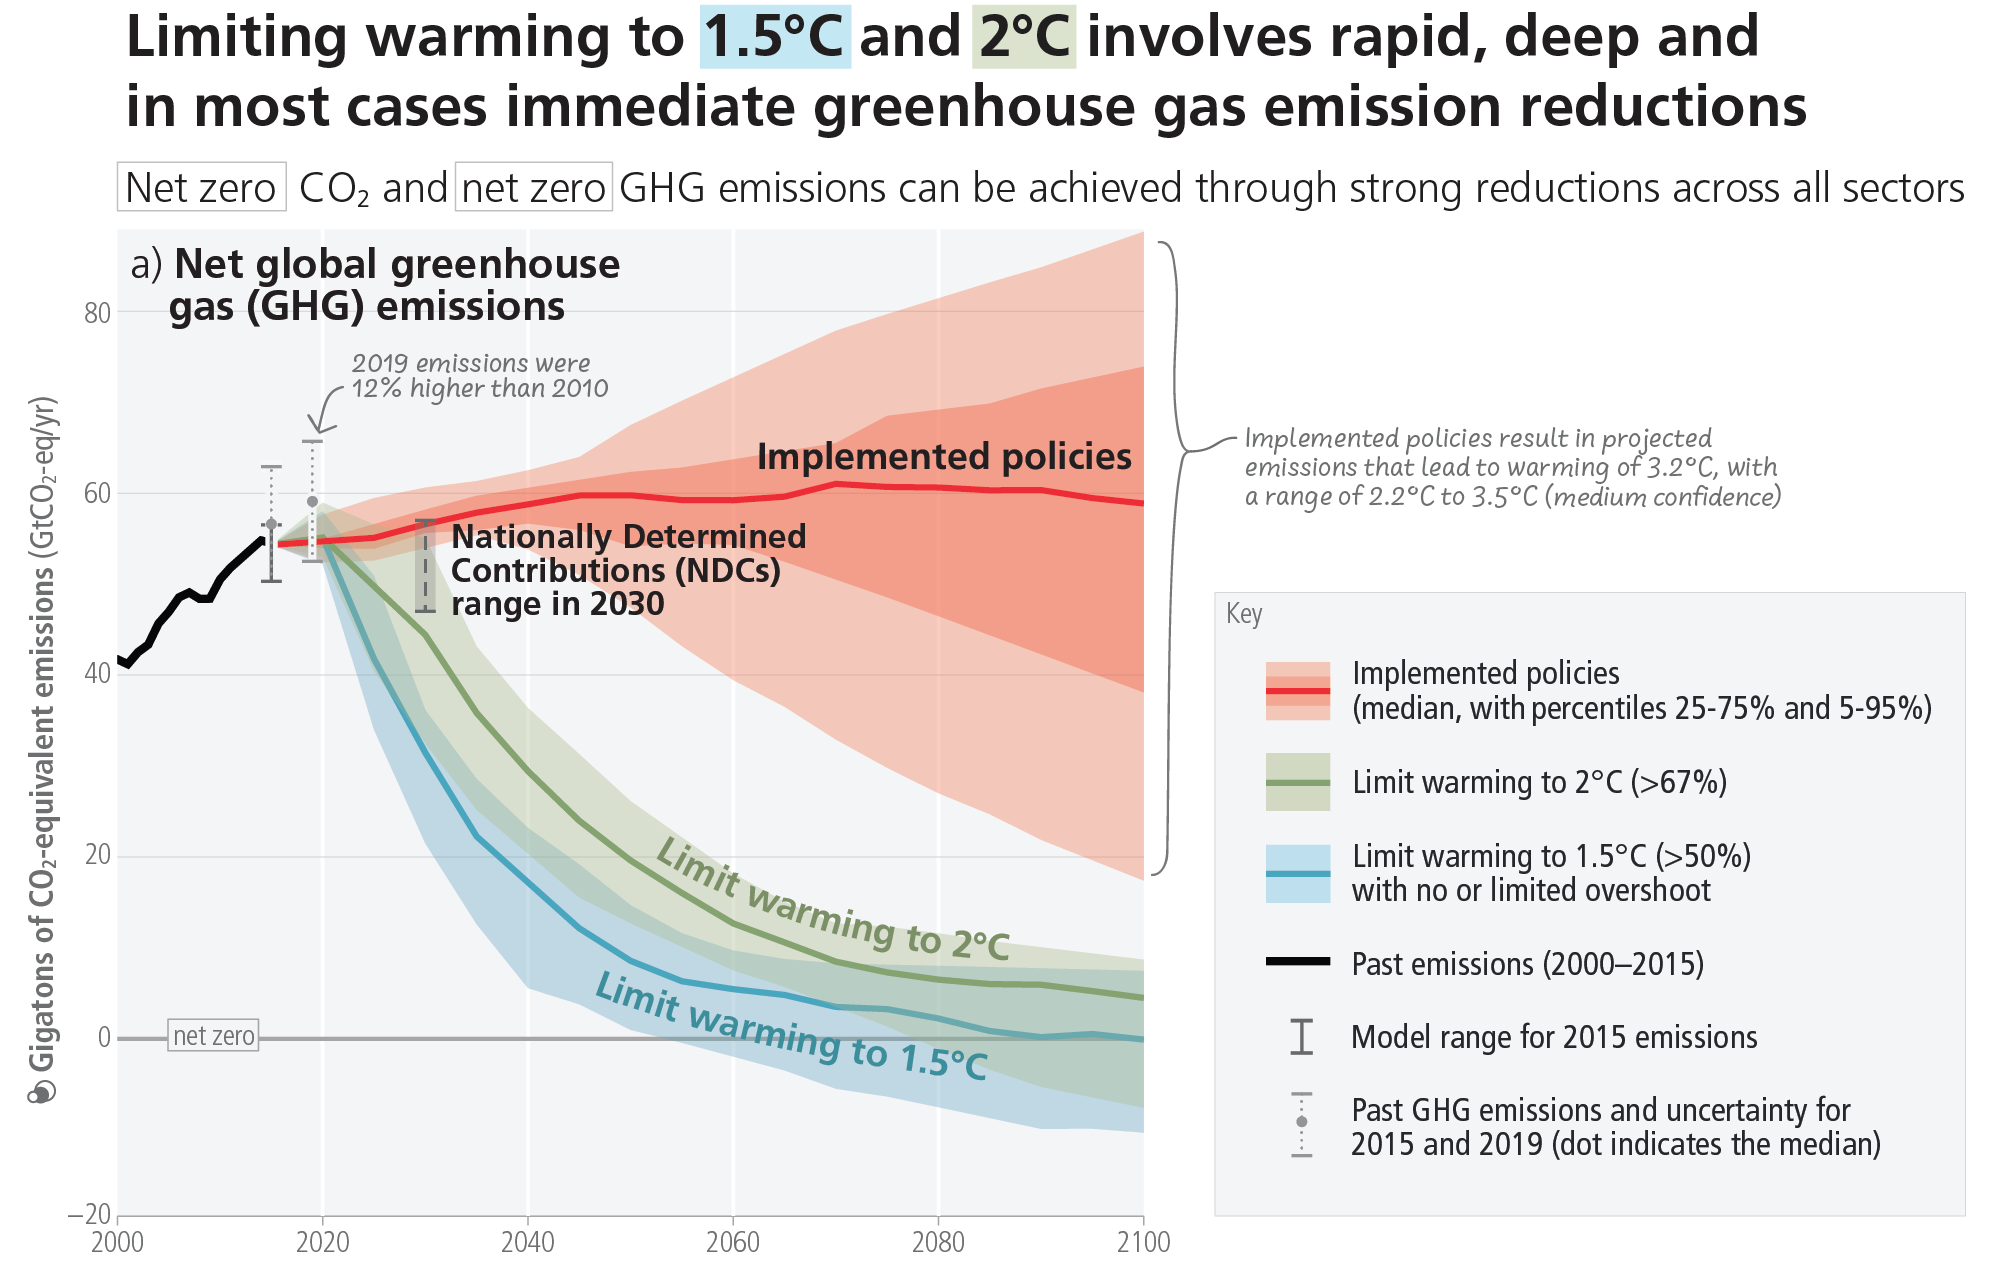
\includegraphics[width=1.00\textwidth]{../Figures/IPCC_AR6_SYR_SPM_Figure5.png}
	\caption{Prognose IPCC (aus \cite{lee_ipcc_2023}) S.22}
	\label{fig:IPCC_AR6_SYR_SPM}
\end{figure}

Abb.~\ref{fig:IPCC_AR6_SYR_SPM} zeigt  die Entwicklung der globalen  CO$_2$-Emissionen in den modellierten Szenarien.  Die roten Bereiche zeigen die Emissionspfade unter der Annahme, dass die Politik bis Ende 2020 umgesetzt wird. Die Bereiche der modellierten Szenarien, die die Erwärmung auf 1,5$^\circ$C ($>$50\%) begrenzen, ohne oder mit begrenzter Überschreitung, sind hellblau dargestellt, und Szenarien, die die Erwärmung auf 2$^\circ$C ($>$67\%) begrenzen, sind grün dargestellt. Globale Emissionspfade, die die Erwärmung auf 1,5$^\circ$C ($>$50\%) begrenzen würden, ohne oder mit begrenzter Überschreitung, und die außerdem in der zweiten Hälfte des Jahrhunderts netto null Treibhausgase erreichen würden, tun dies zwischen 2070 und 2075. Die Treibhausgasemissionen der Vergangenheit für 2010-2015, die für die Projektion der globalen Erwärmungsergebnisse der modellierten Szenarien verwendet wurden, sind durch eine
schwarze Linie dargestellt.


Hier wird eine Diskrepanz zwischen den Darstellungen der IEA und des IPCC über die Auswirkungen und Maßnahmen bezüglich des Klimawandels deutlich. Die Einschätzungen beiden Studien weichen nicht jedoch signifikant von einander  ab,  die Unterschiede liegen  mehr in der Darstellung als im Inhalt, führen aber zu einer anderen Wahrnehmung.


\section{Auswirkungen digitaler Technologien}
Laut der IEA haben digitale Technologien einen signifikanten Einfluss auf die energiebezogenen Treibhausgasemissionen (THG) und trugen im Jahr 2020 mit 2\% zu diesen Emissionen bei. Diese Auswirkungen resultieren direkt aus dem Betrieb von Rechenzentren, Datenübertragungsnetzen und vernetzten Geräten, was zu einem Ausstoß von etwa 330 Megatonnen CO$_2$-Äquivalenten führte, was wiederum 0,9\% der gesamten energiebezogenen THG-Emissionen entspricht.
Trotz des rasanten Wachstums der Nachfrage nach digitalen Dienstleistungen seit 2010 verzeichneten die Emissionen nur eine geringe Steigerung. Dies ist auf verbesserte Energieeffizienz in digitalen Technologien, verstärkten Kauf von erneuerbaren Energien durch Unternehmen im Bereich Informations- und Kommunikationstechnologie (IT) sowie umfassendere Bemühungen zur Dekarbonisierung der Stromnetze zurückzuführen.
Im Szenario der Netto-Null-Emissionen bis 2050 (NZE) ist eine Halbierung der Emissionen bis 2030 erforderlich. Dies stellt eine bedeutende Herausforderung dar und erfordert möglicherweise weiterführende Maßnahmen zur Verringerung des ökologischen Fußabdrucks digitaler Technologien \cite{iea_digitalisation}.

Die Herausforderungen, die sich aus der IT-Infrastruktur und Vernetzung für den Klimawandel ergeben, sind bedeutend. Im Jahr 2020 wurden von Rechenzentren, Datenübertragungsnetzen und vernetzten Geräten insgesamt 330 Megatonnen CO$_2$ emittiert. Diese Zahl verdeutlicht die Notwendigkeit, dass sowohl praktizierende als auch angehende Informatiker sich mit den klimatischen Auswirkungen der IT-Infrastruktur auseinandersetzen sollten.

Trotz einer exponentiellen Steigerung in der Nutzung von Internetdiensten, der Zunahme an Datenzentren und der Verbreitung des Internets der Dinge (IoT), wurde nur eine relativ geringe Zunahme der Emissionen beobachtet. Diese Beobachtung steht im Gegensatz zu früheren Annahmen, wie sie beispielsweise im Shift Report von 2017 getroffen wurden, der von wesentlich höheren Emissionssteigerungen ausging. Nichtsdestotrotz bleibt die Herausforderung bestehen, die Emissionen im Sinne des Netto-Null-Ziels bis 2030 zu halbieren \cite{iea_net_zero2023}.
Demgegenüber steht allerdings der steigenden Energieverbrauch der KI, insbesondere seit 2022 der Large-Language-Modelle, wie ChatGPT \cite{noauthor_ai_nodate}.

\section{Analyse der IT-Infrastruktur in Deutschland}
Die Halbierung der Emissionen stellt eine enorme Aufgabe dar. Wir wollen nun die Situation in Deutschland, betrachten, um konkrete Maßnahmen und Strategien zur Reduktion der Treibhausgasemissionen im Bereich der IT-Infrastruktur und Vernetzung zu diskutieren.
Abb.~\ref{fig:TAB2022_energy demand of ICT} (Abb.~nach \cite{grunwald_energy_2022} S.~2) prognostiziert den Energieverbrauch der IT-Infrastruktur in Deutschland bis 2030.

\begin{figure}[h]
	\centering
		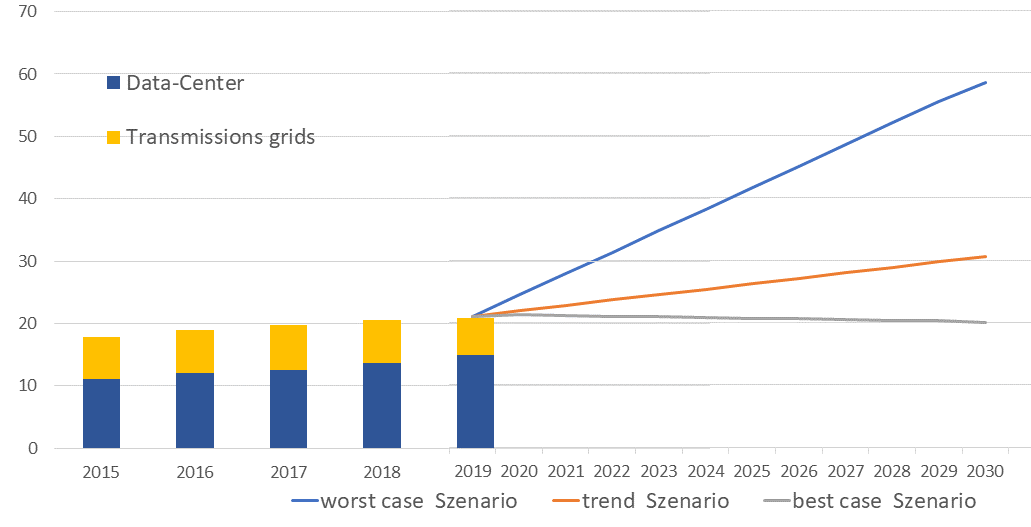
\includegraphics[width=1.00\textwidth]{../Figures/fignachTAB22.png}
		\caption{Szenarien zum Energiebedarf der IT-Infrastruktur bis 2030}
	\label{fig:TAB2022_energy demand of ICT}
\end{figure}


In  \cite{grunwald_energieverbrauch_2022} wird  für den Zeitraum zwischen 2015 und 2019 in Deutschland ein Anstieg des jährlichen Energiebedarfs der IT-Infrastrukturen um knapp 4 TWh festgestellt. Eine eingehende Analyse der IT-Infrastruktur in Deutschland offenbart in Abb.~\ref{fig:TAB2022_energy demand of ICT}  verschiedene Szenarien hinsichtlich des Energieverbrauchs. 
  Die mögliche zukünftige Entwicklung wurde durch die Modellierung von drei Szenarien veranschaulicht (siehe Abb.~\ref{fig:TAB2022_energy demand of ICT}). Im Trendszenario wird erwartet, dass der Energiebedarf von derzeit 21,7 TWh/a bis zum Jahr 2030 auf 30,6 TWh/a steigt. Dies würde einen Anstieg um 70\% gegenüber 2015 bedeuten (bzw. 80\% im Vergleich zu 2010). Im Worst-Case-Szenario könnte der Energiebedarf bis 2030 sogar auf 58,5 TWh/a ansteigen. Das würde eine Verdreifachung des Energiebedarfs der IT-Infrastrukturen in Deutschland im Vergleich zu 2015 bedeuten (bzw. eine Verachtfachung im Vergleich zu 2010). Bei optimaler Ausschöpfung der Effizienzpotenziale im Best-Case-Szenario könnte hingegen eine Stabilisierung und langfristige leichte Absenkung des Energiebedarfs erreicht werden. In diesem Fall würde bis 2030 das Niveau des Energiebedarfs von 2010 wieder erreicht.
	Nichtsdestotrotz ist der Wissensstand zum Energiebedarf der IT-Infrastrukturen unvollständig und teilweise widersprüchlich \cite{grunwald_energieverbrauch_2022}.
	
	Im folgenden wollen wir unseren Blickwinkel weiter einschränken, nämlich darauf was wir als Nutzer einerseits oder als Studierende der Informatik  andererseits ändern können.

\section{Private Internet- und digitale Mediennutzung}
In Deutschland werden  pro Person jährlich rund zwölf Tonnen CO$_2$ durch Energieverbrauch, Verkehr und Konsum  emittiert werden \cite{energieeffizienz_IT_2020}. 
Abb.~\ref{fig:DiagrammCO2Fuss} (siehe auch \cite{infografik_DigFuss_2022}) illustriert, dass  unser digitaler Lebensstil ist für etwa 0,9 Tonnen verantwortlich ist. Nach Angaben des Öko-Instituts ist der Fernseher mit über 350 kg CO$_2$ pro Jahr der größte Verursacher \cite{energieeffizienz_IT_2020}. Auch die Nutzung von Rechenzentren spielt eine große Rolle: Jeder Internetnutzer verursacht rund 213 kg CO$_2$-Emissionen pro Jahr.
Bei der Produktion entstehen Emissionen vor allem durch Prozesschemikalien und den Energieverbrauch. Die Gesamtemissionen eines großen Flachbildfernsehers werden auf 1.000 kg CO 2 geschätzt, die eines Laptops auf 250 kg.
Die nutzungsbedingten Treibhausgasemissionen entstehen vor allem durch den Stromverbrauch der Geräte, der vom Nutzerverhalten abhängt\cite{energieeffizienz_IT_2020}. 

\begin{figure}[h]
	\centering
		\includegraphics[width=.9\linewidth]{../Figures/Diagramm_CO2_Fußabdruck_digitales_Leben.jpg}	
	\caption{\label{fig:DiagrammCO2Fuss} Der CO$_2$-Fußabdruck unseres digitalen Lebens}
\end{figure}


Diese Beobachtungen werfen die Frage auf, welche Maßnahmen wir ergreifen können.
In den letzten Jahres lässt sich die Verlagerung
des Energiebedarfs der privaten Internet- und digitalen Mediennutzung
von den Endgeräten hin zur IT-Infrastruktur beobachten \cite{grunwald_energieverbrauch_2022}. 

Die Übertragung von Daten in Mobilfunknetzen belastet die Umwelt stärker als in kabelgebundenen Breitbandnetzen. Das liegt am größeren CO$_2$-Fußabdruck. 
Fehlanreize sind zum Beispiel Flatrates oder großzügige Datenpakete für Musik- und Videostreaming. Solche Tarife könnten dazu führen, dass Nutzer Videotelefonate über Messenger-Dienste anstelle von Sprachtelefonaten bevorzugen. Videotelefonate verbrauchen etwa fünfmal mehr mobiles Datenvolumen (300 MByte pro Stunde im Vergleich zu 60 MByte pro Stunde) und haben somit einen höheren CO2-Fußabdruck, besonders wenn sie über UMTS-Netze erfolgen.
Weitere Fehlanreize entstehen durch Mobilfunkverträge, die neue Smartphones zu günstigen Preisen anbieten. Die Kosten für die Telefone sind für die Nutzer in den höheren Grundgebühren versteckt. Dies führt dazu, dass Nutzer alle 1 bis 2 Jahre ein neues Smartphone erhalten, was wiederum zu Umweltbelastungen durch Rohstoffverbrauch, Treibhausgasemissionen und Elektronikschrott führt. Stattdessen sollten Mobilfunkverträge die Nutzer mit niedrigen Grundgebühren und nicht subventionierter Hardware dazu ermutigen, ihre Smartphones möglichst lange zu nutzen und so Energie und Ressourcen zu sparen \cite{energieeffizienz_IT_2020}.

In \cite{digitale_leicht_2021} werden folgende Hinweise zum Reduzieren des  digitalen CO$_2$-Fußabdrucks gegeben, die nicht den Verzicht in den Vordergrundstellen.
Die wichtigsten sind:
\begin{itemize}
	\item Längere Nutzung vorhandener Geräte:\\
	    61\% des durchschnittlichen digitalen CO$_2$-Fußabdrucks 
entsteht während der Herstellung, also  beim Abbau
der  Rohstoffe und deren Verarbeitung.  
Second-Hand-Kauf  und Reparaturen sind unterschätzte Möglichkeiten. 
  \item Geräte, wenn möglich ganz ausschalten:\\
	    33\% entstehen durch die  Nutzung digitaler Geräte zu Hause, wobei die Geräte einen guten teil der Zeit nicht genutzt werden, aber dennoch Energie verbrauchen.
			Router, Spielekonsole, Bildschirme haben  im Stand-By einen erstaunlich hohen Verbrauch.
	\item Datenfluss reduzieren:\\
	6\% unserer digitalen CO$_2$-Bilanz resultieren aus dem Datenverkehr bei der Nutzung des Internets. 
	Beispielsweise sind Full HD- und Ultra HD-Videos für 95\% des Datenverkehrs von Video-on-Demand verantwortlich. Eine derart hohe Auflösung ist meistens  überflüssig, weil die Bildqualität nur bei einem sehr großen Bildschirmen dadurch verbessert wird.
\end{itemize}



 Während persönliche Initiativen wie das Ausschalten von Endgeräten über Nacht wichtig und sinnvoll sind, wird deutlich, dass diese allein nicht ausreichen, um den Herausforderungen des Klimawandels zu begegnen. Neben individuellen Maßnahmen sind auch politische und wirtschaftliche Veränderungen entscheidend, um einen signifikanten Einfluss auf die Reduktion von CO$_2$-Emissionen zu erzielen.

Also müssen   politische und wirtschaftliche Hebel in Betracht gezogen werden, um effektive und nachhaltige Lösungen für die Herausforderungen im Bereich der IT-Infrastruktur zu entwickeln. 
Energieeinsparungen im privaten Bereich müssen  obwohl sie einen wichtigen Beitrag leisten, in einem größeren Kontext betrachtet und durch umfassendere Strategien ergänzt werden.





\section{Ansätze in der Softwareentwicklung}
In der Auseinandersetzung mit der Rolle der Informatik im Kontext des Klimawandels wird deutlich, dass etwa ab dem dritten Semester des Informatikstudiums eine zunehmende Fokussierung auf die zukünftigen Herausforderungen und die Verantwortung gegenüber nachfolgenden Generationen erforderlich ist. Die Frage, wie Informatiker*innen  über den Tellerrand hinaus blicken können, ist besonders relevant im Zusammenhang mit den globalen Herausforderungen des Klimawandels.

Die Entwicklung von Software mit möglichst geringer CO$_2$-Emission im gesamten  Lebenszyklus des gesamten Produktes ist ein zunehmend relevantes Thema in der Informatik. Seit den Anfängen der Bewegung für grüne I(K)T  ab 2000, beispielsweise\cite{murugesan_harnessing_2008,uddin_energy_2012}, die sich zunächst auf Energieeinsparungen konzentrierte, hat sich das Feld weiterentwickelt. Ursprünglich durch wirtschaftliche Anreize motiviert, liegt der Fokus nun auch auf der Entwicklung von Software, die über das reine Energiesparen hinausgeht und gleichzeitig ökologischen Mehrwert bietet. Laut \cite{singh_green_2016} begann
\glqq Green  Computing\grqq{}  in den 90er Jahren, als die Umweltschutzbehörde der USA das Energy Star-Programm ins Leben rief. Energy Star ist ein Label-Programm, das Computern und anderen elektronischen Geräten verliehen wird. Es wird grundsätzlich verwendet, um den Energieverbrauch zu minimieren und die Effizienz des Produkts bzw. Geräts zu maximieren. Nach \cite{paul_comprehensive_2023} sind grüne IT und Green  Computing eng miteinander verbundene Konzepte, deren gemeinsames Ziel die Förderung der ökologischen Nachhaltigkeit ist. Grüne IT bezieht sich auf die Nutzung von IT zur Verbesserung der ökologischen Nachhaltigkeit, während sich Green Computing auf das Design, die Entwicklung, die Nutzung und die Entsorgung von Computersystemen in einer umweltverträglichen Weise konzentriert.


Wir wollen uns jetzt mit den Ansätzen  zu CO$_2$-effiziente Softwareentwicklung befassen.
Es existieren zahlreiche Ansätze unter verschiedenen Bezeichnungen (Grüne IT, Green Computation, grüne, nachhaltige, ressourcen-effiziente SW etc.), um CO$_2$-Effizienz in der Softwareentwicklung zu erreichen. Dabei wird aber in den meisten Fällen nur als Ziel genannt, Software zu entwickeln, die sowohl für Nutzer einen Mehrwert bietet als auch den CO$_2$-Ausstoß minimiert.

Die Diskussion um CO$_2$-effiziente Software wirft allerdings auch kritische Fragen auf, insbesondere in Bezug auf den kommerziellen Sektor. Während der Fokus auf der Reduzierung von CO$_2$-Emissionen liegt, wird die Sinnhaftigkeit der umfassenden digitalen Anwendungen oft nicht hinterfragt. Dies führt zu einer Diskrepanz zwischen dem Streben nach CO$_2$-Effizienz und der umfassenden Bewertung der Notwendigkeit und des Nutzens digitaler Produkte. Solche Ansätze stehen können auch zum  Greenwashing betragen, einer Praxis, bei der Unternehmen umweltfreundliche Maßnahmen behaupten, die möglicherweise nicht der Realität entsprechen. 
Es ist daher wichtig, kritisch zu hinterfragen und sorgfältig zu prüfen, inwieweit solche Maßnahmen tatsächlich zur CO$_2$-Effizienz und Ressourcenschonung beitragen.

Die meisten Geschäftsmodelle hinter der Massendigitalisierung erfordern eine ständige Zunahme des Inhalts- und Datenverbrauchs sowie der
Infrastruktur, um langfristig rentabel zu bleiben \cite{brouillard_deploying_2021}. 
 Weitergehende  Ansätze, die die Frage nach der grundsätzliche Sinnhaftigkeit der Produkte stellen, sind beispielsweise das Konzept der \glqq Digitalen Nüchternheit\grqq{} (digital sobriety) \cite{project_shift_2019,brouillard_deploying_2021}, welches die Notwendigkeit hinterfragt, ob alle vorhandenen digitalen Anwendungen tatsächlich benötigt werden. 

Auch das Konzept der digitalen Suffizienz (\cite{santarius_digital_2023}) bildet eine Grundlage, um zu verstehen, wie die IT Teil des grundlegenden ökologischen Wandels werden können und besteht aus vier Dimensionen 
\begin{itemize}
	\item Hardwaresuffizienz: die darauf abzielt, dass weniger Geräte produziert werden müssen und ihr absoluter Energiebedarf so gering wie möglich gehalten wird, um die gewünschten Aufgaben zu erfüllen.
  \item  Softwaresuffizienz, die darauf abzielt, dass der Datenverkehr und die Hardwareauslastung während der Anwendung so gering wie möglich gehalten werden; 
 \item Nutzersuffizienz, die darauf abzielt, dass die Nutzer digitale Geräte sparsam einsetzen und die IT in einer Weise nutzen, die einen nachhaltigen Lebensstil fördert; und 
\item Ökonomische Suffizienz, die darauf abzielt, dass die Digitalisierung den Übergang zu einer Wirtschaft unterstützt, die nicht durch Wirtschaftswachstum als primäres Ziel, sondern durch ausreichende Produktion und ausreichenden Verbrauch innerhalb der planetarischen Grenzen gekennzeichnet ist. 
\end{itemize}




\section{CO$_2$-Effizienz und Ressourcenschonung}

Ansätze zur CO$_2$-Effizienz und der Ressourcenschonung in der Softwareentwicklung umfassen Überlegungen zur Notwendigkeit und Effizienz von Software sowie deren Auswirkungen auf den Hardwarebedarf und die Umwelt. Der Fokus liegt auf der Entwicklung von Software, die nicht nur energieeffizient ist, sondern auch die Notwendigkeit von häufigen Hardware-Aktualisierungen reduziert.

Eine ressourcenschonende Software wird charakterisiert durch ihre Fähigkeit, auf bestehender Hardware zu laufen und dadurch den Bedarf an neuen Geräten zu verringern. Diese Abwärtskompatibilität und längere Nutzungsdauer führen zu einer höheren Energieeffizienz und geringeren Umweltbelastung. Es wird auch festgestellt, dass Open-Source-Software im Allgemeinen energieeffizienter ist als proprietäre Software.

Verschiedene Initiativen wie die Green Software Foundation\footnote{%
             siehe \href{https://greensoftware.foundation/}{https://greensoftware.foundation/})},%
an der Unternehmen wie Microsoft teilnehmen, und SAPs CleanIT\footnote{%
       siehe \href{https://open.sap.com/courses/cleanit2021-hpi}{https://open.sap.com/courses/cleanit2021-hpi}}, %
sind Beispiele für Bemühungen in dieser Richtung. 

Die Reduktion von CO$_2$-Emissionen und Stromverbrauch in der Informationstechnologie umfasst verschiedene Ansätze, die sowohl die Hardware-Herstellung als auch den Betrieb berücksichtigen. Ein wesentlicher Aspekt ist das verdinglichte CO$_2$, welches bereits bei der Herstellung von Hardware entsteht. Die Minimierung der Hardwareproduktion und die Verlängerung ihrer Lebensdauer tragen signifikant zur CO$_2$-Einsparung bei.

Darüber hinaus spielt die Nutzung von erneuerbaren Energien eine entscheidende Rolle. Indem Aufgaben und Datenverarbeitung in Datencentern mit erneuerbaren Energien verlagert werden, kann der CO$_2$-Ausstoß reduziert werden. Google plant, seine Rechenzentren bis 2030 ausschließlich mit kohlenstofffreier
Energie zu betreiben\cite{Google_2020}. 
Je nach Energiequellen und Nachfrage schwankt die Kohlenstoffintensität des öffentlichen Stromnetzes im Laufe der Zeit. Die Ausnutzung dieser Schwankungen ist ein wichtiger Faktor für die Verringerung der von Rechenzentren verursachten Emissionen. Dabei gibt es einerseits  die CO$_2$-bewusste Verlagerung von Arbeitslasten über geografisch verteilte Rechenzentren hinweg \cite{yang_carbon-neutralized_2022}, und andererseits  die  Verlagerung von Rechenlasten auf Zeiten, in denen die Energieversorgung voraussichtlich weniger kohlenstoffintensiv ist, z.B in  \cite{wiesner_lets_2021}.
Dies erfordert jedoch eine kritische Betrachtung des Datenverkehrs, da auch dieser Ressourcen verbraucht. Die Energieproportionalität \cite{abts_energy_2010, zheng_distributed_2022} ist hier ein wichtiges Konzept, welches besagt, dass Server und Netzwerkinfrastrukturen effizient genutzt werden sollten, um unnötigen CO$_2$-Verbrauch zu vermeiden. 
Energieproportionalität bezieht sich auf das Verhältnis von Energieverbrauch zu Rechenlast, wobei die Energieeffizienz mit zunehmender Last steigt. Das bedeutet, dass ein Server, selbst wenn er keine Berechnungen durchführt, immer noch einen signifikanten Prozentsatz der Energie verbraucht, die er unter Höchstlast benötigen würde.

Beispielsweise kann ein Server, der von 10\% auf 40\% seiner Berechnungskapazität skaliert, den Energieverbrauch nur um den Faktor 1,7 erhöhen. Dies unterstreicht die Effizienz des Cloud-Computings, insbesondere wenn Datenzentren auf erneuerbare Energiequellen setzen. Große Anbieter wie Microsoft, Google und AWS bewerben ihre Bemühungen um grüne IT, obwohl ein gewisser Grad an Greenwashing vorhanden sein mag. 
Ein weiterer relevanter Aspekt ist die Power Usage Efficiency (PUE) für Datenzentren. PUE misst, wie viel des verbrauchten Stroms tatsächlich für Berechnungen verwendet wird und wie viel als Overhead anfällt. Die Optimierung der PUE ist nicht nur aus ökologischen, sondern auch aus kommerziellen Gründen wichtig, da geringerer Stromverbrauch zu niedrigeren Betriebskosten führt.


\section{Messung von Energieverbrauch und Laufzeit}

Es gibt im groben drei Parameter, die, unabhängig von der Infrastruktur, die die CO$_2$-Emissionen beeinflussen:
der aktuelle oder auch der durchschnittliche  Energieverbrauch, der  Energie-Mix aus erneuerbaren und fossilen Energiequellen und die Menge und Art der Hardware.

Im folgenden untersuchen wir die Messung des Energieverbrauchs. Die These lautet: 
\begin{center}
Was nicht gemessen werden kann, kann auch nicht verbessert werden. 
\end{center}
Daher ist es entscheidend, den tatsächlichen Stromverbrauch zu erfassen, um ihn effektiv reduzieren zu können. Diese Ansätze sind sowohl im Kontext der CO$_2$-effizienten Softwareentwicklung als auch im Netzwerkmanagement relevant.

Die Frage des Energieverbrauchs bei der Softwareentwicklung ist komplex, da der Energiemix und die verwendete Hardware oft nicht direkt vom Entwickler steuerbar sind. Dennoch ist es möglich, den Energieverbrauch der Software durch spezifische Implementierungen zu beeinflussen. Verschiedene Tools können eingesetzt werden, um den Energieverbrauch zu messen, und diese Messungen können wichtige Erkenntnisse für die Entwicklung energieeffizienter Software liefern.

Die Messung des Energieverbrauchs  stellt eine Herausforderung dar, die verschiedene Ansätze erfordert. Die direkte Messung des Stromverbrauchs an der Steckdose ist eine Möglichkeit, jedoch kann sie nicht immer die genaue Menge des Verbrauchs bestimmen, insbesondere bei batteriebetriebenen Geräten. Hardware-basierte Tests können kostspielig und aufwändig sein, daher bieten Software-Tools eine alternative Möglichkeit zur Überwachung des Energieverbrauchs.
Verschiedene Überwachungstools, wie JoularX und PowerJoular\footnote{%
   siehe  \href{https://www.noureddine.org/research/joular/joularjx}{https://www.noureddine.org/research/joular/joularjx}} \cite{noureddine-ie-2022}, bieten Schnittstellen zur Messung des Energieverbrauchs. Andere Tools, wie der Software-Footprint\footnote{%
   siehe  \href{https://github.com/oekoj/softwarefootprint}{https://github.com/oekoj/softwarefootprint}} nutzen Prozessstatistiken, und Intels PowerGadget\footnote{%
   siehe \href{https://www.intel.com/content/www/us/en/developer/articles/tool/power-gadget.html}{https://www.intel.com/content/www/us/en/developer/articles/tool/power-gadget.html}}  bietet Funktionen zur Integration in Code-Abschnitte. Diese Tools müssen auf die spezifischen Bedürfnisse und die verfügbare Hardware der Nutzer abgestimmt werden.
Die Komplexität der Messung wird durch Faktoren wie die Auslastung von Hintergrundprogrammen erhöht, die nicht direkt zur laufenden Applikation gehören, aber dennoch den Energieverbrauch beeinflussen können. Dies unterstreicht die Wichtigkeit, den Gesamtbetrieb auf der Hardware zu berücksichtigen und bei Bedarf zu reduzieren, um genaue Messungen zu ermöglichen. 


Energieeffizienz bezieht sich auf die verbrauchte Energie eines Systems \cite{brown_toward_2010} und definiert
sie durch die minimale Menge an Energie, die das System benötigt um eine Aufgabe auszuführen.
Laufzeiteffizienz bezieht sich auf die Geschwindigkeit und Leistung von Computersystemen, die Komplexität von Algorithmen und die Qualität der Implementierung.
In der historischen Betrachtung der Informatik war die Laufzeiteffizienz von Algorithmen aufgrund begrenzter CPU-Kapazitäten und Speicherplatz ein zentrales Anliegen. Diese Priorität führte zur Entwicklung von Algorithmen, die primär auf minimale Laufzeit ausgerichtet waren. Die Frage ist nun, ob es einen Zusammenhang zwischen Energieeffizienz und Laufzeiteffizienz gibt. 



Die Untersuchung der Korrelation zwischen Energieverbrauch und Laufzeit ist Gegenstand aktueller Forschung.
Manche Arbeiten \cite{pereira_energy_2017,cascaval_folklore_2014,pinto_energy_2017} deuten darauf hin, dass in vielen Fällen eine starke Korrelation besteht, was impliziert, dass energieeffiziente Software oft auch laufzeiteffizient ist. Falls es einen direkten Zusammenhang zwischen Energieeffizienz und Performance gibt  könnte eine Laufzeitmessung ausreichend sein und legt nahe, dass die Fokussierung auf Laufzeiteffizienz in der Informatik indirekt auch zur Energieeffizienz beiträgt.

Andere Arbeiten  \cite{trefethen_energy-aware_2013,lima_haskell_2016}, weisen keine direkte Proportionalität zwischen verbesserter Laufzeit und verringertem  Energieverbrauch. Eine Verbesserung in der Laufzeiteffizienz bedeutet nicht zwangsläufig eine Verbesserung in der Energieeffizienz und umgekehrt.
Falls kein direkter Zusammenhang besteht, sind  unabhängige  Messungen  des Energieverbrauchs erforderlich. 



\section{Computer Science for Future}

Die Initiative \href{https://cs4f.de}{Computer Science for Future} setzt sich für Initiativen im Bereich Klimaschutz und Nachhaltigkeit aus der Perspektive der Informatik ein. Dabei streben wir an, diese Initiativen in verschiedene Bereiche zu integrieren:

\begin{itemize}
	\item Integration in das Curriculum, um Studierende mit relevanten Kenntnissen auszustatten.
	\item Zusammenarbeit mit Industrie- und Gesellschaftspartnern, um praxisnahe Lösungen zu entwickeln.
	\item Integration in die Forschung, um innovative Ansätze für nachhaltige Technologien zu erforschen.
	\item Implementierung in die organisatorischen Abläufe, um einen ganzheitlichen Ansatz zu gewährleisten.
\end{itemize}
Getragen wird diese Initiative von engagierten Personen, darunter Studierende, Mitarbeiterinnen und Professorinnen, die den Wandel hin zu nachhaltigen Praktiken in der Informatik vorantreiben möchten.


\printbibliography %Prints bibliography%

\end{document}
